\section{آدرس‌دهی و مدیریت حافظه در فایل‌های PE}
\label{sec:pe_addressing}

یکی از مهم‌ترین مفاهیم در درک ساختار فایل‌های PE و مهندسی معکوس، نحوه آدرس‌دهی و نگاشت فایل از دیسک به حافظه است. فایل‌های اجرایی روی دیسک ساختاری فشرده دارند، اما هنگام اجرا در حافظه، برای رعایت الزامات سیستم‌عامل و سخت‌افزار (مانند Paging)، ساختار آن‌ها تغییر می‌کند. درک تفاوت بین آدرس‌های فایل (Raw) و آدرس‌های حافظه (Virtual) برای تحلیلگران بدافزار و مهندسان معکوس حیاتی است.

\subsection{انواع آدرس‌ها}

در تحلیل فایل‌های PE با سه نوع آدرس اصلی مواجه هستیم:

\begin{enumerate}
    \item \textbf{آدرس مجازی (\lr{Virtual Address - VA}):}
    آدرس مطلق یک دستورالعمل یا داده در حافظه مجازی فرآیند. این آدرس همان چیزی است که پردازنده (CPU) هنگام اجرای برنامه می‌بیند. برای مثال، اگر یک دستور در آدرس \texttt{0x401000} قرار داشته باشد، مقدار \texttt{EIP/RIP} به این آدرس اشاره می‌کند.
    
    \item \textbf{آدرس مجازی نسبی (\lr{Relative Virtual Address - RVA}):}
    آدرس یک آیتم نسبت به نقطه شروع بارگذاری فایل در حافظه (\lr{Image Base}). فایل‌های PE معمولاً از RVA استفاده می‌کنند تا مستقل از محل بارگذاری باشند (\lr{Relocatable}). رابطه بین VA و RVA به صورت زیر است:
    \begin{equation}
    VA = \text{Image Base} + RVA
    \end{equation}
    
    \item \textbf{آدرس خام یا آفست فایل (\lr{Raw Address / File Offset}):}
    موقعیت فیزیکی داده‌ها درون فایل ذخیره‌شده روی دیسک. وقتی فایلی را با یک \lr{Hex Editor} باز می‌کنید، با این آدرس‌ها سر و کار دارید.
\end{enumerate}

\subsection{هم‌ترازی (\lr{Alignment})}
یکی از دلایل تفاوت بین آدرس‌های روی دیسک و حافظه، مفهوم هم‌ترازی است.

\begin{itemize}
    \item \textbf{\lr{File Alignment}:} برای کاهش فضای دیسک، بخش‌های فایل روی دیسک معمولاً با مضرب‌های کوچک‌تری (مثلاً ۲۰۰ هگزادسیمال یا ۵۱۲ بایت) هم‌تراز می‌شوند.
    \item \textbf{\lr{Section Alignment}:} در حافظه، به دلیل معماری مدیریت حافظه سیستم‌عامل (Paging)، بخش‌ها باید با مضرب‌های بزرگ‌تری (معمولاً ۱۰۰۰ هگزادسیمال یا ۴۰۹۶ بایت) هم‌تراز شوند.
\end{itemize}

این تفاوت باعث می‌شود که فاصله بین بخش‌ها در حافظه بیشتر از دیسک باشد و در نتیجه، موقعیت نسبی داده‌ها تغییر کند.

\subsection{نگاشت فایل به حافظه (\lr{Mapping})}
تصویر زیر تفاوت چیدمان بخش‌ها در فایل (دیسک) و حافظه را نشان می‌دهد. توجه کنید که چگونه بخش‌ها در حافظه «کشیده» می‌شوند.

\begin{center}
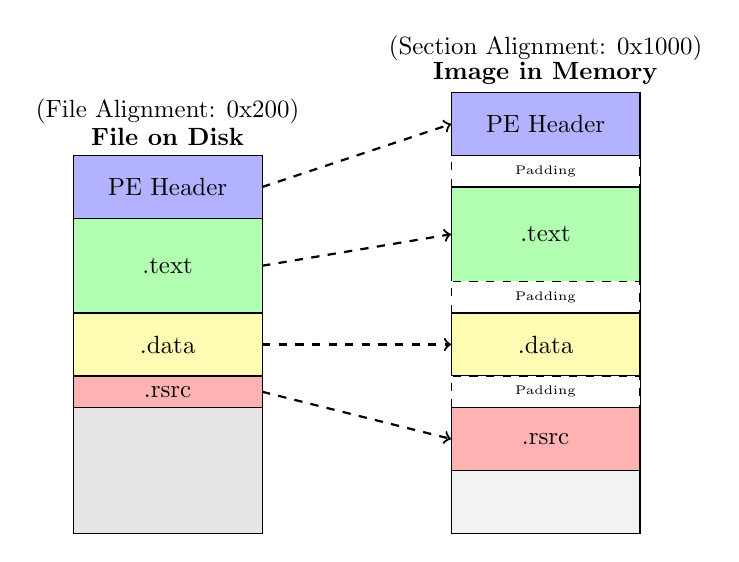
\begin{tikzpicture}[scale=0.8, every node/.style={scale=0.9}]
    % Disk View
    \draw[fill=gray!20] (0,0) rectangle (3,6);
    \node at (1.5, 6.3) {\textbf{File on Disk}};
    \node at (1.5, 6.7) {(File Alignment: 0x200)};
    
    \draw[fill=blue!30] (0,5) rectangle (3,6) node[midway] {PE Header};
    \draw[fill=green!30] (0,3.5) rectangle (3,5) node[midway] {.text};
    \draw[fill=yellow!30] (0,2.5) rectangle (3,3.5) node[midway] {.data};
    \draw[fill=red!30] (0,2) rectangle (3,2.5) node[midway] {.rsrc};
    
    % Memory View
    \draw[fill=gray!10] (6,0) rectangle (9,7);
    \node at (7.5, 7.3) {\textbf{Image in Memory}};
    \node at (7.5, 7.7) {(Section Alignment: 0x1000)};
    
    \draw[fill=blue!30] (6,6) rectangle (9,7) node[midway] {PE Header};
    \draw[fill=white, dashed] (6,5.5) rectangle (9,6) node[midway, font=\tiny] {Padding};
    
    \draw[fill=green!30] (6,4) rectangle (9,5.5) node[midway] {.text};
    \draw[fill=white, dashed] (6,3.5) rectangle (9,4) node[midway, font=\tiny] {Padding};
    
    \draw[fill=yellow!30] (6,2.5) rectangle (9,3.5) node[midway] {.data};
    \draw[fill=white, dashed] (6,2) rectangle (9,2.5) node[midway, font=\tiny] {Padding};
    
    \draw[fill=red!30] (6,1) rectangle (9,2) node[midway] {.rsrc};
    
    % Arrows
    \draw[->, thick, dashed] (3,5.5) -- (6,6.5);
    \draw[->, thick, dashed] (3,4.25) -- (6,4.75);
    \draw[->, thick, dashed] (3,3) -- (6,3);
    \draw[->, thick, dashed] (3,2.25) -- (6,1.5);

\end{tikzpicture}
\end{center}

\subsection{محاسبه آدرس خام (\lr{RVA to Raw Offset})}
برای یافتن محل یک داده در فایل (هنگامی که آدرس حافظه آن را داریم)، باید مراحل زیر را طی کنیم:

\begin{enumerate}
    \item \textbf{یافتن بخش مربوطه:} بررسی کنید که RVA مورد نظر در محدوده کدام بخش قرار دارد.
    \[ \text{Section.VirtualAddress} \le RVA < \text{Section.VirtualAddress} + \text{Section.VirtualSize} \]
    \item \textbf{محاسبه اختلاف:} فاصله RVA از ابتدای آن بخش را محاسبه کنید.
    \[ \text{Delta} = RVA - \text{Section.VirtualAddress} \]
    \item \textbf{اعمال به فایل:} این اختلاف را به آفست خام آن بخش اضافه کنید.
    \[ \text{Raw Offset} = \text{Section.PointerToRawData} + \text{Delta} \]
\end{enumerate}

\subsection{مثال عملی}
فرض کنید اطلاعات زیر را از هدرهای یک فایل PE استخراج کرده‌ایم:

\begin{table}[ht]
\centering
\caption{اطلاعات بخش‌های یک فایل نمونه}
\begin{tabular}{|c|c|c|c|}
\hline
\textbf{Section} & \textbf{Virtual Address (RVA)} & \textbf{Virtual Size} & \textbf{Pointer to Raw Data} \\
\hline
.text & 0x1000 & 0x500 & 0x400 \\
\hline
.data & 0x2000 & 0x300 & 0xA00 \\
\hline
\end{tabular}
\end{table}

اگر بخواهیم بدانیم آدرس حافظه \texttt{0x401020} (با فرض \lr{ImageBase = 0x400000}) در کجای فایل روی دیسک قرار دارد:

\begin{enumerate}
    \item \textbf{محاسبه RVA:}
    \[ RVA = 0x401020 - 0x400000 = 0x1020 \]
    \item \textbf{یافتن بخش:} مقدار \texttt{0x1020} بزرگتر از \texttt{0x1000} (.text) و کوچکتر از \texttt{0x2000} (.data) است. پس این آدرس متعلق به بخش \textbf{.text} است.
    \item \textbf{محاسبه آفست:}
    \[ \text{Raw Offset} = 0x400 + (0x1020 - 0x1000) = 0x400 + 0x20 = 0x420 \]
\end{enumerate}

بنابراین، اگر فایل را در \lr{Hex Editor} باز کنیم، بایت‌های مربوط به این دستور را در آفست \texttt{0x420} خواهیم یافت.
